
% 1 : x; 2: y; 3: tikz object name
\newcommand\nocnode[3]{
    \node[circle, draw, color=black, anchor=south, thick, minimum size=1cm, inner sep=0pt] (r#3) at (#1, #2) {#3};
}

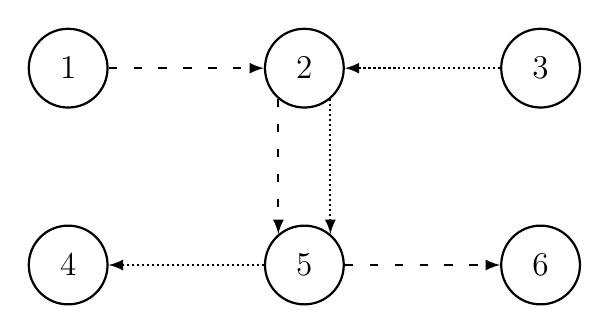
\begin{tikzpicture}[font={\fontsize{12pt}{12}\selectfont}]
    
    \nocnode{0}{0}{1}
    \nocnode{3}{0}{2}
    \nocnode{6}{0}{3}
    \nocnode{0}{-2.5}{4}
    \nocnode{3}{-2.5}{5}
    \nocnode{6}{-2.5}{6}

    \draw[-latex, thick, loosely dashed] (r1) -- (r2);
    \draw[-latex, thick, loosely dashed] (r2.230) -- (r5.130);
    \draw[-latex, thick, loosely dashed] (r5) -- (r6);

    \draw[-latex, thick, densely dotted] (r3) -- (r2);
    \draw[-latex, thick, densely dotted] (r2.310) -- (r5.50);
    \draw[-latex, thick, densely dotted] (r5) -- (r4);

\end{tikzpicture}
